\begin{frame}{Context}{Collective Adaptive System (CAS) working group}
\begin{figure}
	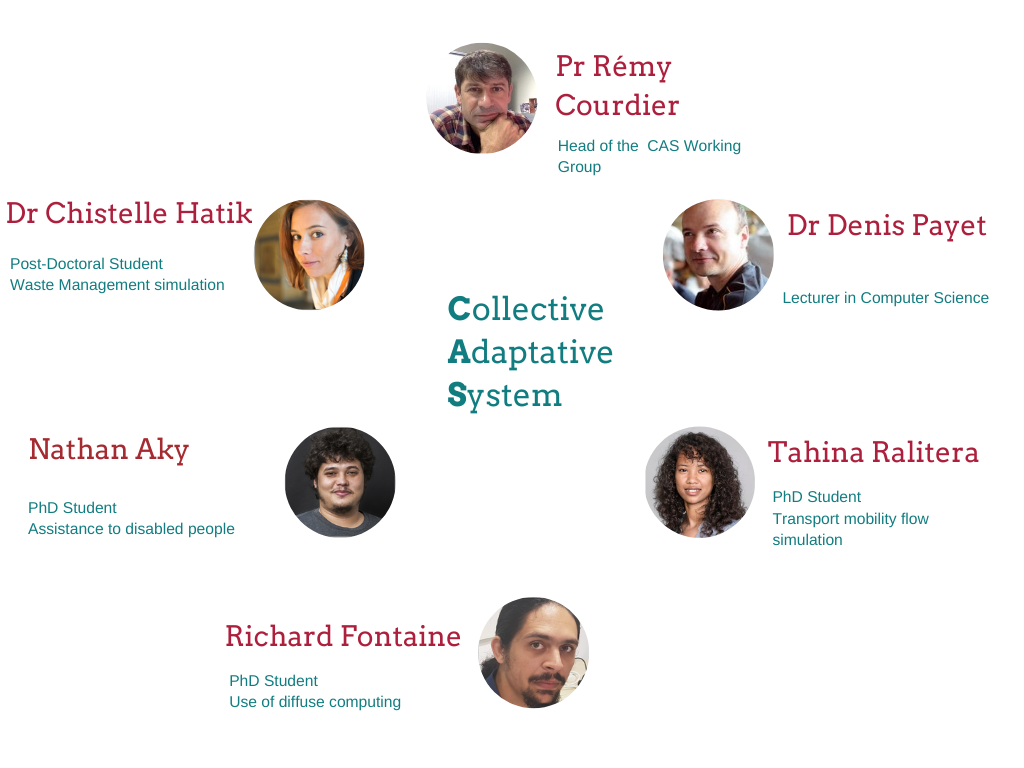
\includegraphics[width=.8\textwidth]{figures/SCA.png}
\end{figure}
\note{Cette thèse s’inscrit dans la continuité des travaux étudiés précédemment par le groupe de travail SCA du LIM qui se compose actuellement des personnes suivantes. Le groupe est spécialisé dans le paradigme des SMA.
}
\end{frame}

\begin{frame}{Context}{Collective Adaptive System (CAS) working group}
\par Our team is specialized in the field of Multi-Agent Systems: 
\begin{itemize}
    \item Bottom-up approach
    \item The intelligence emerge from the agents interaction with the environment
\end{itemize}
\begin{figure}
	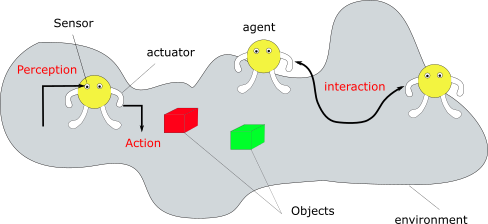
\includegraphics[width=.6\textwidth]{figures/SMA.png}
\end{figure}
\par Current team orientation: Towards hybrid approaches (simulation and real environment application)
\par However, \alert{my thesis focuses on multi-agent simulation (MAS)}

\note{Par définition, un système multi-agent est un système composé d'un ensemble d'objets et d'agents situés dans un certain environnement et interagissant selon certaines relations. Un agent est une entité autonome et pro-active. Il est doté de capteurs qui lui permet de percevoir son environnement et d'actionneurs qui lui permet d'agir sur ce dernier. La modélisation à base de SMA est une approche ascendante. L'intelligence émerge alors de l'interaction entre les agents et l'environnement.
\par Notre équipe s'est focalisé depuis plus de 20 ans sur la simulation multi-agents. Néanmoins notre politique actuelle s’oriente plus vers les approches de type hybrides. C’est-à-dire nous nous intéresson à la fois à la simulation et à l’application dans un environnement réel. Ainsi, bien que dans le cadre de cette thèse, je me concentre essentiellement sur la simulation, je prends tout de même en compte dans mes choix l’éventualité d’une future implémentation en milieu réel.
}
\end{frame}


\begin{frame}{Context}{Multi-agent simulations of smart cities and smart islands}
\textbf{Sub-theme}: Application of multi-agent simulations in the field of smart cities and smart islands. Collaboration with 
    \begin{figure}
	
\includegraphics[width=2cm]{assets/icl.png}
	\hspace{2cm}
	
\includegraphics[width=1cm]{assets/saintDenis.png}
    \end{figure}

\begin{block}{Smart City}
Using ICTs to solve the problems related to growing urbanization, the economic and environmental crisis that cities are currently facing and which put pressure on their structure and on the \textbf{resources management}. 

\begin{itemize}
    \item The citizen participates proactively in the system 
    \item Bottom-up approach
    \item Participatory intelligence that emerges from interactions between the citizen and the system
\end{itemize}
\alert{MAS approach is a promising approach for smart city systems modeling}
\end{block}
\note{
Un des sous-thèmes que nous développons consiste en la simulation multi-agent appliquée aux villes intelligentes et aux îles intelligentes. Ma thèse s'inscrit dans ce contexte. Il s’agit d’un domaine en émergence dans notre équipe et sur lequel nous travaillons en collaboration avec des chercheurs de l'ICL et avec la mairie de Saint-Denis, La Réunion.

Comme il n'y a pas encore de standard permettant de définir ce qu'est une ville intelligente, nous aimerions clarifier notre vision de ce qu'est une ville intelligente que nous partageaons avec d'autres scientifiques travaillant dans le domaine. Le concept de smart city est considéré comme étant une solution technique qui consiste à utiliser les TIC pour résoudre les problèmes liés à l’urbanisation croissante, la crise économique et environnementale auxquelles les villes font actuellement face et qui mettent une pression sur leur structure et sur la gestion des ressources. Nous tenons également à noter que nous accordons une grande importance à la place qu'occupe le citoyen au sein du système. Le citoyen n'est pas vu comme un simple utilisateur qui subit le système, il y participe de manière proactive. L'intelligence dont il est sujet ici est alors une forme d'intelligence participative qui émerge des interactions entre les citoyens et les citoyens et le système. L'approche multi-agents est notamment une approche prometteuse permettant la modélisation de ce type de système.
}
    
\end{frame}


\begin{frame}{Context}{Multi-agent simulations of smart cities and smart islands}
\textbf{Sub-theme}: Multi-agent simulation of smart cities and smart islands. Collaboration with 
    \begin{figure}
	
\includegraphics[width=2cm]{assets/icl.png}
	\hspace{2cm}
	
\includegraphics[width=1cm]{assets/saintDenis.png}
    \end{figure}

\alert{Focus on smart mobility} : Multi-agent simulation of electric vehicles flow movement in a territory. Example : London and Reunion Island
    \begin{itemize}
        \item \textbf{SkuadCityModel} : built upon the SimSKUAD platform, developed within our team
        \item \textbf{SmartCityModel} : built upon the Repast Simphony platform, developed by ICL, contribution of our team (2 scientific articles)
    \end{itemize}

\note{
Les problématiques abordées sont en lien avec la mobilité intelligente. Nous menons nos expérimentations sur un modèle de simulation multi-agent de flux de déplacement de véhicules électriques sur un territoire que nous développons au sein même de notre équipe. Ce modèle s’appelle SkuadCityModel. Il se base sur un modèle développé par les chercheurs de l’ICL appelé SmartCityModel, sur lequel nous avons également contribué et qui a fait l'objet de deux publications. Les problématiques abordées dans le cadre de cette thèse découlent des limites détectées lors de ces expérimentations. SmartCityModel tourne sur la plateforme internationale Repast Simphony tandis que SkuadCityModel tourne sur une plateforme que nous avons développé appelée SimSKUAD.
}
    
\end{frame}

%%%%%%%%%%%%%%%%%%%%%%%%%%%%%%%%%%%%%%%%%%%%%%%%%

\begin{frame}{Problem}
\textbf{Example}\footnote{https://www.flaticon.com/}: 
\begin{figure}
	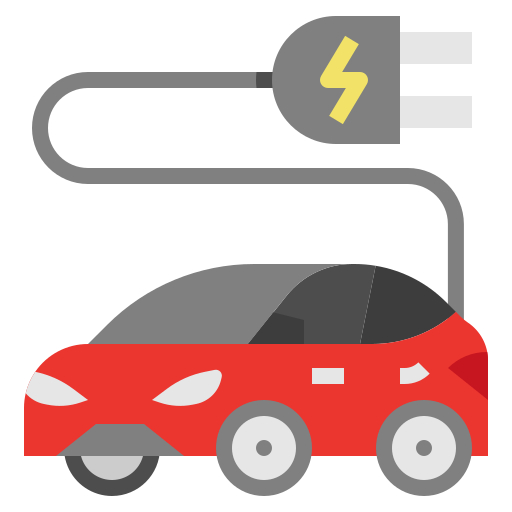
\includegraphics[width=1.8cm]{figures/electric-car.png}
	\hspace{2cm}
	
\includegraphics[width=1.8cm]{figures/charging.png}
\end{figure}
\textbf{Objective}: optimise the management of vehicle recharging with public charging points

\textbf{Problem}: management of shared and limited resources in space and \textbf{time}
\par 2 complementary needs:
\begin{itemize}
    \item A need for interaction support for the exchange of spatial, temporal and social information
    \item A need for reasoning that allows to take into account this exchanged information
\end{itemize}

\note{
L’exemple sur lequel nous nous basons est celui du rechargement des véhicules électriques avec des bornes de recharge publiques. L'objectif est d'optimiser la gestion du rechargement des véhicules. Cet exemple illustre un problème plus général qui est la gestion d'une ressource partagée et limitée dans l'espace et dans le temps. Cette dernière fait partie des problèmes à l’origine même de la création du concept de ville intelligente que j’ai énoncé précédemment. Nous nous intéressons particulièrement à la prise en compte de la dimension temporelle. Il s'agit d'une dimension qui contrairement à la dimension spatiale, dans les SMA, reste sujette à très peu d’étude et de considération.
\par Une première étude autour de ce sujet nous a permis de relever deux besoins complémentaires sur lesquels nous apportons notre contribution :
\begin{itemize}
    \item Un besoin en support d'interaction pour l'échange d'informations spatiales, temporelles et sociales;
    \item Un besoin en raisonnement permettant de prendre en compte ces informations échangées dans l'objectif d'optimiser la gestion de ressources partagées et limitées dans l'espace et le temps.
\end{itemize}
}
    
\end{frame}

\begin{frame}{Problem}
\textbf{Problem}: management of shared and limited resources in space and \textbf{time}
\par Space is subject to a lot of studies, we decide to look at the consideration of the time as a model dynamic
\par We distinguish 2 aspects of time:
\begin{itemize}
    \item \textbf{Time (temporal information) representation}. Space, time and organization are the 3 important dimensions in the study of territorial systems \footnote{Rolland-May, C. (2000). Évaluation des territoires: concepts, modèle, méthodes. Hermès science publications.}. However, \alert{the temporal dimension (temporal dynamics) is often neglected}.
    \vspace{.5cm}
    \item \textbf{Temporal reasoning}. Taking into account past, present and future information in anticipatory reasoning is natural to humans. However, \alert{in most multi-agent simulations, agents consider only past and present information in their reasoning}.
\end{itemize}

\note{\footnotesize{
\par Après avoir établi un état de l'art autour des besoins cités précédemment, nous avons conclu que notre problématique relève de la non-prise en compte du temps simulé en tant que dynamique du modèle dans les SMA. Dans notre réflexion, nous distinguons deux aspects de ce temps simulé : la représentation du temps et le raisonnement temporel. Chaque aspect nous permet de répondre à chacun des besoins énoncés précédemment.
\par L’espace, le temps et les organisations sont les 3 dimensions qui selon Rolland May devraient être intégrés au même titre dans l’étude des systèmes territoriaux. Cependant, dans les sma, contrairement à la dimension spatiale et la dimension sociale qui font l’objet de nombreuses propositions dans la littérature, la considération du temps comme une dynamique du système reste sujette à très peu d’étude et de considération. \par L'exploitation des informations spatiales ou organisationnelles est classique dans le raisonnement anticipatif dans les sma. Dans SmartCityModel et SkuadCityModel, cela consiste par exemple à utiliser la minimisation de la distance prévisionnelle entre la localisation actuelle du véhicule et de sa destination, la prise en compte de la pente comme critère de choix entre plusieurs destinations possibles. Cet exemple illustre la prise en compte des 3 dimensions de l'environnement spatial: abscisse, ordonnée et hauteur dans le raisonnement anticipatif qui semble très naturelle. 
\par La conception du temps linéaire est également définie sur 3 positions : le passé, le présent et le futur. Cependant, à notre connaissance, la majorité des mécanismes d'anticipation utilise dans leur modèle prédictif des informations positionnées uniquement sur le passé et sur le présent. Ces informations sont utilisées pour générer des prédictions (sur le futur). Pourtant, chez l'humain, la prise en compte des informations sur ces 3 dimensions du temps dans le processus de raisonnement anticipatif est naturelle chez l'humain.}}
    
\end{frame}

\begin{frame}{Contributions}
A set of solutions on 2 aspects:
\begin{itemize}
    \item \textbf{Time representation}: a medium that allows the exchange of temporal information on the same basis as spatial information and social information
    \item \textbf{Temporal reasoning}: exploit the spatial, the temporal and the social information exchanged through the medium in the context of anticipatory reasoning
\end{itemize}
\note{
Afin de nous affranchir des limites citées précédemment, au niveau de
\begin{itemize}
    \item La représentation du temps : nous proposons de mettre en place un support permettant l’échange d’informations temporel au même titre que les informations spatiales et sociales
    \item Le raisonnement temporel : nous proposons un raisonnement anticipatif qui en plus des informations spatiales, sociales et sur les dimensions passées et présentes du temps, exploite aussi la dimension future du temps. Cela est permis par le support mis en place au niveau de la représentation du temps qui offre une visibilité sur la dimension future du temps.
\end{itemize}
La mise en place de ces deux contributions au sein de notre système devrait permettre d’optimiser la gestion des ressources partagées dans l’espace et dans le temps, en offrant notemment une visibilité sur une dimension futur du temps que nous exploitons dans le raisonnement anticipatif de l'agent.
Cependant, avant de rentrer plus en détails dans les contributions et pour une meilleure compréhension, je vais vous expliquer brièvement le fonctionnement général d’une simulation multi-agents avec un focus particulier sur la gestion du temps.
}
\end{frame}